\documentclass[
  10pt,
  aspectratio=169,
  utf8,
  xcolor={dvipsnames}
]{beamer}

\usetheme[
  progressbar=foot,
  sectionpage=progressbar,
  subsectionpage=progressbar,
  numbering=fraction
]{metropolis}
\usefonttheme{metropolis}
\usecolortheme{spruce}
\setbeamercolor{progress bar}{fg=MidnightBlue, bg=LightSteelBlue}
\setbeamercolor{title}{fg=MidnightBlue}
\setbeamercolor{frame title}{fg=MidnightBlue}
\setbeamercolor{structure}{fg=MidnightBlue}

\usepackage{booktabs}
\usepackage{graphicx}
\usepackage{tikz}
\usetikzlibrary{shapes, arrows, positioning, fit, backgrounds}
\usepackage{amsmath}
\usepackage{amssymb}
\usepackage{fontspec}
\usepackage{caption}
\captionsetup[figure]{labelformat=empty}
\captionsetup[table]{labelformat=empty}

\title{\textbf{Maximum Likelihood Estimation and Logistic Regression}}
\subtitle{Quantitative \& Modeling - SDS6210 Informatics for Health}
\author{\textbf{Cavin Otieno}}
\institute{Department of Public Health\\University}
\date{\today}

\begin{document}

% Group Members Frame
{
\setbeamertemplate{footline}{}
\begin{frame}
\titlepage
\end{frame}
}

\begin{frame}{Group 5 Members}
\begin{center}
\begin{tabular}{ll}
\toprule
\textbf{Student ID} & \textbf{Student Name} \\
\midrule
SDS6/46982/2024 & Cavin Otieno \\
SDS6/47543/2024 & Laura Nabalayo Kundu \\
SDS6/47659/2024 & John Andrew \\
\bottomrule
\end{tabular}
\end{center}
\end{frame}

\begin{frame}{Outline}
\tableofcontents
\end{frame}

% ============================================================================
% SECTION 1: INTRODUCTION TO MAXIMUM LIKELIHOOD ESTIMATION
% ============================================================================

\section{Maximum Likelihood Estimation: Foundational Concepts}

\subsection{What is Maximum Likelihood Estimation?}

\begin{frame}{The Problem of Statistical Estimation}
Statistical inference involves estimating unknown parameters from observed data:

\begin{block}{The Estimation Problem}
Given a random sample $X_1, X_2, \ldots, X_n$ from a distribution with probability density function $f(x|\theta)$, where $\theta$ is an unknown parameter, we seek to estimate $\theta$ based on the observed data.
\end{block}

\begin{center}
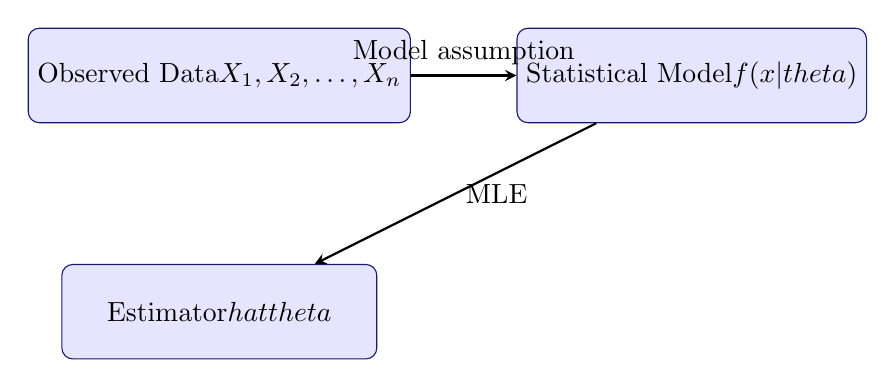
\begin{tikzpicture}[node distance=2cm]
\tikzstyle{block} = [rectangle, rounded corners, minimum width=4cm, minimum height=1.2cm, text centered, draw=MidnightBlue, fill=blue!10]
\tikzstyle{arrow} = [thick,->,>=stealth]

\node (data) [block] {Observed Data\\$X_1, X_2, \ldots, X_n$};
\node (model) [block, right of=data, xshift=4cm] {Statistical Model\\$f(x|\\theta)$};
\node (estimate) [block, below of=data, yshift=-1cm] {Estimator\\$\\hat{\\theta}$};

\draw [arrow] (data) -- (model) node[midway, above] {Model assumption};
\draw [arrow] (model) -- (estimate) node[midway, right] {MLE};
\end{tikzpicture}
\end{center}
\end{frame}

\begin{frame}{Definition of Maximum Likelihood Estimation}
Maximum Likelihood Estimation (MLE) is a fundamental method for estimating statistical parameters:

\begin{block}{Fundamental Principle}
The likelihood function measures the plausibility of different parameter values given the observed data. The MLE is the parameter value that makes the observed data most probable (most likely).
\end{block}

\begin{definition}[Likelihood Function]
Given a sample $X_1 = x_1, X_2 = x_2, \ldots, X_n = x_n$ from a distribution with pdf $f(x|\theta)$, the likelihood function is:
$$L(\theta) = L(\theta|x_1, x_2, \ldots, x_n) = \prod_{i=1}^{n} f(x_i|\theta)$$
\end{definition}

\begin{block}{Maximum Likelihood Estimator}
The MLE $\hat{\theta}$ is the value of $\theta$ that maximizes the likelihood function:
$$\hat{\theta} = \arg\max_{\theta} L(\theta)$$
\end{block}
\end{frame}

\begin{frame}{Example: Bernoulli Distribution}
Consider estimating the success probability $p$ from Bernoulli trials:

\begin{block}{Problem Setup}
Suppose we observe $n$ independent Bernoulli trials with success probability $p$:
$$X_i \sim \text{Bernoulli}(p), \quad P(X_i = x) = p^x(1-p)^{1-x}, \quad x \in \{0,1\}$$
\end{block}

\begin{block}{Likelihood Function}
The likelihood for observing $y$ successes in $n$ trials is:
$$L(p) = P(\text{Data}|p) = p^y(1-p)^{n-y}$$
where $y = \sum_{i=1}^{n} x_i$ is the total number of successes.
\end{block}

\begin{block}{MLE Solution}
To find the MLE, we maximize $L(p)$:
$$\frac{d}{dp}L(p) = y p^{y-1}(1-p)^{n-y} - (n-y)p^y(1-p)^{n-y-1} = 0$$
Solving yields $\hat{p} = \frac{y}{n}$, the sample proportion.
\end{block}
\end{frame}

\begin{frame}{Example: Normal Distribution}
For normally distributed data, the MLE has a familiar form:

\begin{block}{Problem Setup}
Let $X_1, \ldots, X_n \sim \mathcal{N}(\mu, \sigma^2)$. The pdf is:
$$f(x_i|\mu,\sigma^2) = \frac{1}{\sqrt{2\pi\sigma^2}} \exp\left(-\frac{(x_i-\mu)^2}{2\sigma^2}\right)$$
\end{block}

\begin{block}{Likelihood Function}
$$L(\mu,\sigma^2) = \prod_{i=1}^{n} \frac{1}{\sqrt{2\pi\sigma^2}} \exp\left(-\frac{(x_i-\mu)^2}{2\sigma^2}\right)$$
\end{block}

\begin{block}{MLE Results}
\begin{align*}
\hat{\mu} &= \bar{X} = \frac{1}{n}\sum_{i=1}^{n} X_i \\
\hat{\sigma}^2 &= \frac{1}{n}\sum_{i=1}^{n}(X_i - \bar{X})^2
\end{align*}
Note: $\hat{\sigma}^2$ is biased (uses $n$ instead of $n-1$).
\end{block}
\end{frame}

\subsection{The Log-Likelihood Function}

\begin{frame}{Why Use the Log-Likelihood?}
The log-likelihood transformation simplifies maximization:

\begin{block}{Log-Likelihood Definition}
$$\ell(\theta) = \log L(\theta) = \log \left(\prod_{i=1}^{n} f(x_i|\theta)\right) = \sum_{i=1}^{n} \log f(x_i|\theta)$$
\end{block}

\begin{center}
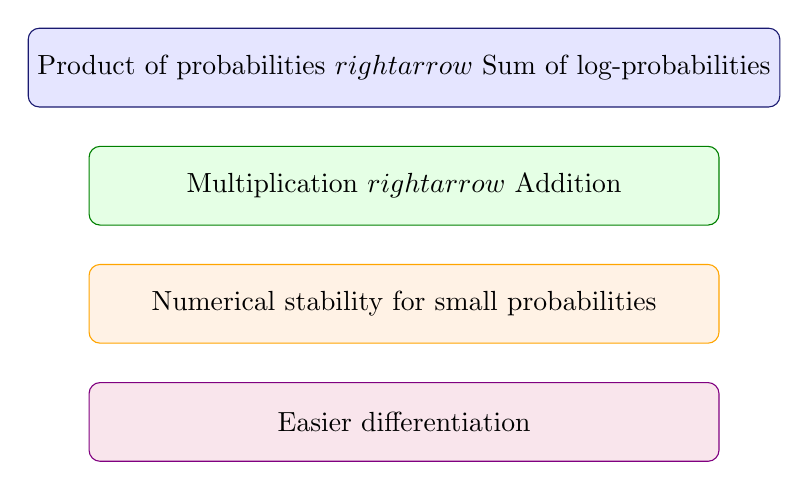
\begin{tikzpicture}[node distance=1.5cm]
\tikzstyle{transform} = [rectangle, rounded corners, minimum width=8cm, minimum height=1cm, text centered]

\node (T1) [transform, draw=MidnightBlue, fill=blue!10] {Product of probabilities $\\rightarrow$ Sum of log-probabilities};
\node (T2) [transform, below of=T1, draw=Green, fill=green!10] {Multiplication $\\rightarrow$ Addition};
\node (T3) [transform, below of=T2, draw=Orange, fill=orange!10] {Numerical stability for small probabilities};
\node (T4) [transform, below of=T3, draw=Purple, fill=purple!10] {Easier differentiation};
\end{tikzpicture}
\end{center}
\end{frame}

\begin{frame}{Log-Likelihood: Bernoulli Example}
Returning to the Bernoulli example:

\begin{block}{Log-Likelihood Function}
\begin{align*}
\ell(p) &= \log\left[p^y(1-p)^{n-y}\right] \\
        &= y\log p + (n-y)\log(1-p)
\end{align*}
\end{block}

\begin{block}{Maximization}
Taking the derivative:
$$\frac{d\ell}{dp} = \frac{y}{p} - \frac{n-y}{1-p} = 0$$
Solving gives $\hat{p} = \frac{y}{n}$, confirming our previous result.
\end{block}

\begin{block}{Second Derivative (Hessian)}
$$\frac{d^2\ell}{dp^2} = -\frac{y}{p^2} - \frac{n-y}{(1-p)^2} < 0$$
Since the second derivative is negative, $\hat{p}$ is a maximum.
\end{block}
\end{frame}

\begin{frame}{Properties of MLE Estimators}
MLE possesses several desirable statistical properties:

\begin{columns}
\begin{column}{0.5\textwidth}
\begin{block}{Consistency}
As sample size $n \rightarrow \infty$, $\hat{\theta}_n \xrightarrow{p} \theta$, meaning the estimator converges in probability to the true parameter value.
\end{block}
\begin{block}{Asymptotic Normality}
For large $n$, $\hat{\theta} \approx \mathcal{N}(\theta, \text{Var}(\hat{\theta}))$, where the variance can be estimated from the Fisher information.
\end{block}
\end{column}
\begin{column}{0.5\textwidth}
\begin{block}{Asymptotic Efficiency}
The MLE achieves the Cramér-Rao lower bound asymptotically, meaning it has the smallest possible variance among consistent estimators.
\end{block}
\begin{block}{Invariance Property}
If $\hat{\theta}$ is the MLE of $\theta$, then $g(\hat{\theta})$ is the MLE of $g(\theta)$ for any function $g(\cdot)$.
\end{block}
\end{column}
\end{columns}
\end{frame}

% ============================================================================
% SECTION 2: LOGISTIC REGRESSION FOUNDATIONS
% ============================================================================

\section{Logistic Regression: The Binary Outcome Model}

\subsection{Why Logistic Regression?}

\begin{frame}{Limitations of Linear Regression for Binary Outcomes}
When the outcome variable is binary ($Y \in \{0,1\}$), linear regression is problematic:

\begin{block}{Problems with Linear Probability Model}
$$P(Y=1|X) = \beta_0 + \beta_1 X_1 + \cdots + \beta_k X_k$$
\begin{itemize}
\item Predicted probabilities can be $< 0$ or $> 1$
\item Heteroscedasticity: Variance depends on $X$ ($Var(Y|X) = p(1-p)$)
\item Error terms are not normally distributed
\end{itemize}
\end{block}

\begin{center}
\begin{tikzpicture}[node distance=2cm]
\tikzstyle{plot} = [rectangle, rounded corners, minimum width=6cm, minimum height=4cm, draw=gray]

\node (P1) at (-3,0) [plot] {};
\node (P2) at (3,0) [plot] {};

\node at (-3,2.5) {Linear Model};
\node at (3,2.5) {Logistic Model};

\draw[->, thick] (-4.5,-1) -- (-1.5,-1) node[right] {$X$};
\draw[->, thick] (-4.5,-1) -- (-4.5,1.5) node[above] {$P(Y=1|X)$};

\draw[->, thick] (1.5,-1) -- (4.5,-1) node[right] {$X$};
\draw[->, thick] (1.5,-1) -- (1.5,1.5) node[above] {$P(Y=1|X)$};

\draw[domain=-3:-1.5, samples=10, thick, red] plot ({sin(deg(\x))});
\draw[domain=1.5:4.5, samples=20, thick, blue] plot ({0.5*tanh(\x-3)});
\end{tikzpicture}
\end{center}
\end{frame}

\begin{frame}{The Logistic Function}
The logistic (sigmoid) function transforms linear predictors to probabilities:

\begin{block}{Logistic (Sigmoid) Function}
$$\pi(z) = \frac{1}{1 + e^{-z}} = \frac{e^z}{1 + e^z}$$
where $z$ is the linear predictor and $\pi(z) \in (0,1)$ for all $z \in \mathbb{R}$.
\end{block}

\begin{block}{Key Properties}
\begin{itemize}
\item $\pi(-z) = 1 - \pi(z)$ (symmetry)
\item $\pi(0) = 0.5$ (median effective dose)
\item As $z \rightarrow \infty$, $\pi(z) \rightarrow 1$
\item As $z \rightarrow -\infty$, $\pi(z) \rightarrow 0$
\end{itemize}
\end{block}

\begin{center}
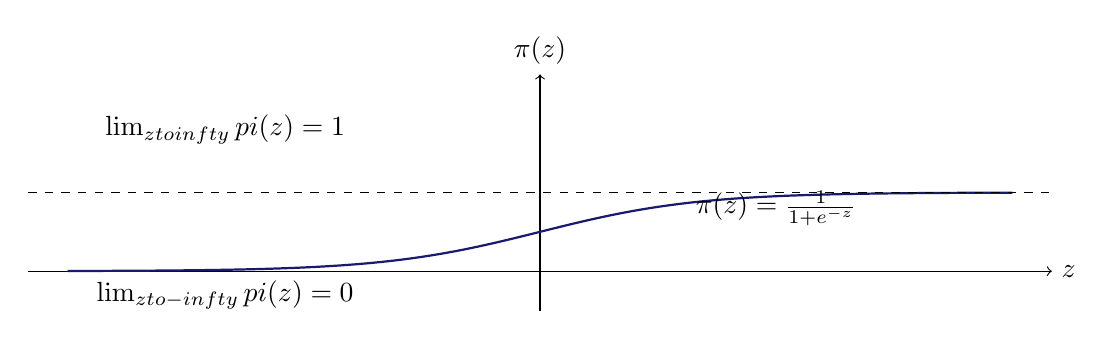
\begin{tikzpicture}[domain=-6:6, smooth, samples=100]
\draw[->] (-6.5,0) -- (6.5,0) node[right] {$z$};
\draw[->] (0,-0.5) -- (0,2.5) node[above] {$\pi(z)$};

\draw[thick, MidnightBlue] plot (\x, {1/(1+exp(-\x))});
\draw[dashed] (-6.5,1) -- (6.5,1);
\draw[dashed] (0,1) -- (0,1.1);

\node at (3,0.8) {$\pi(z) = \frac{1}{1+e^{-z}}$};
\node at (-4,1.8) {$\lim_{z \\to \\infty} \\pi(z) = 1$};
\node at (-4,-0.3) {$\lim_{z \\to -\\infty} \\pi(z) = 0$};
\end{tikzpicture}
\end{center}
\end{frame}

\begin{frame}{The Logistic Regression Model}
Logistic regression models the log-odds as a linear function of predictors:

\begin{block}{Probability Model}
For a binary outcome $Y \in \{0,1\}$ and covariates $X_1, X_2, \ldots, X_k$:
$$P(Y=1|X) = \frac{1}{1 + e^{-(\beta_0 + \beta_1 X_1 + \cdots + \beta_k X_k)}}$$
\end{block}

\begin{block}{Log-Odds Form (Logit)}
Taking the log-odds (logit transformation):
\begin{align*}
\log\left(\frac{P(Y=1|X)}{1-P(Y=1|X)}\right) &= \beta_0 + \beta_1 X_1 + \cdots + \beta_k X_k
\end{align*}
This linearizes the model while constraining probabilities to $(0,1)$.
\end{block}

\begin{block}{Odds Interpretation}
The ratio $\frac{P(Y=1|X)}{1-P(Y=1|X)}$ represents the odds of the outcome. Logistic regression models the log-odds as a linear function of predictors.
\end{block}
\end{frame}

\begin{frame}{Assumptions of Logistic Regression}
\begin{columns}
\begin{column}{0.5\textwidth}
\begin{block}{Model Assumptions}
\begin{itemize}
\item Binary outcome (Bernoulli distribution)
\item Linearity in the log-odds
\item Independence of observations
\item No perfect multicollinearity
\end{itemize}
\end{block}
\end{column}
\begin{column}{0.5\textwidth}
\begin{block}{Link Function}
The logit link function connects the linear predictor to the response mean:
$$g(\mu) = \log\left(\frac{\mu}{1-\mu}\right) = X\beta$$
where $\mu = E(Y|X) = P(Y=1|X)$.
\end{block}
\end{column}
\end{columns}

\begin{block}{Generalized Linear Model Framework}
Logistic regression is a Generalized Linear Model (GLM) with:
\begin{itemize}
\item \textbf{Distribution:} Binomial/Bernoulli
\item \textbf{Link function:} Logit (log-odds)
\end{itemize}
\end{block}
\end{frame}

% ============================================================================
% SECTION 3: LIKELIHOOD DERIVATION FOR LOGISTIC REGRESSION
% ============================================================================

\section{Deriving the Likelihood for Logistic Regression}

\subsection{Constructing the Likelihood Function}

\begin{frame}{Data Structure for Logistic Regression}
Let the observed data consist of $n$ independent observations:

\begin{block}{Notation}
For each observation $i = 1, \ldots, n$:
\begin{itemize}
\item $Y_i \in \{0, 1\}$: Binary outcome
\item $X_i = (1, X_{i1}, X_{i2}, \ldots, X_{ik})$: Vector of predictors (including intercept)
\item $\beta = (\beta_0, \beta_1, \ldots, \beta_k)^T$: Vector of regression coefficients
\end{itemize}
\end{block}

\begin{block}{Probability Model for Observation $i$}
\begin{align*}
P(Y_i = 1|X_i, \beta) &= \pi_i = \frac{1}{1 + e^{-X_i^T\beta}} \\
P(Y_i = 0|X_i, \beta) &= 1 - \pi_i = \frac{e^{-X_i^T\beta}}{1 + e^{-X_i^T\beta}}
\end{align*}
where $\pi_i = P(Y_i = 1|X_i, \beta)$.
\end{block}
\end{frame}

\begin{frame}{Individual Observation Likelihood}
The probability mass function for observation $i$ is:

\begin{block}{Bernoulli PMF for Logistic Regression}
$$P(Y_i = y_i|X_i, \beta) = \pi_i^{y_i}(1 - \pi_i)^{1 - y_i}, \quad y_i \in \{0,1\}$$
where $\pi_i = \frac{1}{1 + e^{-X_i^T\beta}}$.
\end{block}

This can be written more compactly using the logit formulation:

\begin{block}{Alternative Formulation}
\begin{align*}
P(Y_i = y_i|X_i, \beta) &= \frac{\exp(y_i \cdot X_i^T\beta)}{1 + \exp(X_i^T\beta)}
\end{align*}
This form is often more convenient for derivations.
\end{block}
\end{frame}

\begin{frame}{The Likelihood Function for Logistic Regression}
Since observations are assumed independent, the likelihood is the product of individual probabilities:

\begin{block}{Likelihood Function}
$$L(\beta) = \prod_{i=1}^{n} P(Y_i = y_i|X_i, \beta) = \prod_{i=1}^{n} \pi_i^{y_i}(1 - \pi_i)^{1 - y_i}$$
where $\pi_i = \frac{1}{1 + e^{-X_i^T\beta}}$.
\end{block}

\begin{block}{Substituting the Alternative Form}
$$L(\beta) = \prod_{i=1}^{n} \frac{\exp(y_i \cdot X_i^T\beta)}{1 + \exp(X_i^T\beta)}$$
\end{block}

\begin{block}{Key Challenge}
The likelihood function is nonlinear in $\beta$, and there is no closed-form solution for $\hat{\beta}$. Numerical optimization methods are required.
\end{block}
\end{frame}

\begin{frame}{The Log-Likelihood Function}
Taking the log of the likelihood simplifies the product to a sum:

\begin{block}{Log-Likelihood Derivation}
\begin{align*}
\ell(\beta) &= \log L(\beta) \\
            &= \sum_{i=1}^{n} \log\left[P(Y_i = y_i|X_i, \beta)\right] \\
            &= \sum_{i=1}^{n} \left[y_i \log \pi_i + (1 - y_i) \log(1 - \pi_i)\right]
\end{align*}
\end{block}

\begin{block}{Alternative Form}
\begin{align*}
\ell(\beta) &= \sum_{i=1}^{n} \left[y_i X_i^T\beta - \log(1 + \exp(X_i^T\beta))\right]
\end{align*}
\end{block}

\begin{block}{Goal}
Find $\hat{\beta}$ that maximizes $\ell(\beta)$:
$$\hat{\beta} = \arg\max_{\beta} \ell(\beta)$$
\end{block}
\end{frame}

\begin{frame}{Log-Likelihood: Binary Prediction Example}
Consider a simple case with no predictors (intercept-only model):

\begin{block}{Model}
$$P(Y_i = 1) = \pi = \frac{1}{1 + e^{-\beta_0}}$$
\end{block}

\begin{block}{Log-Likelihood}
$$\ell(\beta_0) = \sum_{i=1}^{n} \left[y_i \beta_0 - \log(1 + e^{\beta_0})\right]$$
For $n_1$ ones and $n_0$ zeros:
$$\ell(\beta_0) = n_1 \beta_0 - n \log(1 + e^{\beta_0})$$
\end{block}

\begin{block}{MLE Solution}
Differentiating and setting to zero:
$$\frac{d\ell}{d\beta_0} = n_1 - n \frac{e^{\beta_0}}{1 + e^{\beta_0}} = 0 \implies \hat{\pi} = \frac{n_1}{n}$$
Thus $\hat{\beta}_0 = \log\left(\frac{n_1/n}{1 - n_1/n}\right) = \log\left(\frac{n_1}{n_0}\right)$, the log-odds.
\end{block}
\end{frame}

\begin{frame}{The Score Function (First Derivative)}
To find the MLE, we set the score function to zero:

\begin{block}{Score Vector Definition}
The score function (gradient) is the vector of first partial derivatives:
$$U(\beta) = \frac{\partial \ell(\beta)}{\partial \beta} = \left(\frac{\partial \ell}{\partial \beta_0}, \ldots, \frac{\partial \ell}{\partial \beta_k}\right)^T$$
\end{block}

\begin{block}{Score Function Derivation}
\begin{align*}
\frac{\partial \ell}{\partial \beta_j} &= \sum_{i=1}^{n} \frac{\partial}{\partial \beta_j} \left[y_i X_i^T\beta - \log(1 + e^{X_i^T\beta})\right] \\
                                        &= \sum_{i=1}^{n} \left[y_i X_{ij} - \frac{X_{ij} e^{X_i^T\beta}}{1 + e^{X_i^T\beta}}\right] \\
                                        &= \sum_{i=1}^{n} X_{ij} (y_i - \pi_i)
\end{align*}
where $\pi_i = \frac{e^{X_i^T\beta}}{1 + e^{X_i^T\beta}}$.
\end{block}

\begin{block}{Score Equations}
$$U_j(\beta) = \sum_{i=1}^{n} X_{ij}(y_i - \pi_i) = 0, \quad j = 0, 1, \ldots, k$$
\end{block}
\end{frame}

\begin{frame}{The Hessian Matrix (Second Derivative)}
The Hessian matrix provides information about curvature and is used in optimization:

\begin{block}{Hessian Definition}
$$\mathbf{H}(\beta) = \frac{\partial^2 \ell(\beta)}{\partial \beta \partial \beta^T}$$
\end{block}

\begin{block}{Second Derivative Derivation}
\begin{align*}
\frac{\partial^2 \ell}{\partial \beta_j \partial \beta_l} &= \frac{\partial}{\partial \beta_l} \sum_{i=1}^{n} X_{ij}(y_i - \pi_i) \\
                                                          &= -\sum_{i=1}^{n} X_{ij} X_{il} \frac{\partial \pi_i}{\partial \beta_l} \\
                                                          &= -\sum_{i=1}^{n} X_{ij} X_{il} \pi_i (1 - \pi_i)
\end{align*}
since $\frac{\partial \pi_i}{\partial \beta_l} = X_{il} \pi_i (1 - \pi_i)$.
\end{block}

\begin{block}{Hessian Matrix}
$$\mathbf{H}(\beta) = -\mathbf{X}^T \mathbf{W} \mathbf{X}$$
where $\mathbf{W} = \text{diag}\{\pi_1(1-\pi_1), \ldots, \pi_n(1-\pi_n)\}$ is the weight matrix.
\end{block}
\end{frame}

% ============================================================================
% SECTION 4: NUMERICAL ESTIMATION OF COEFFICIENTS
% ============================================================================

\section{Numerical Optimization for MLE}

\subsection{Iterative Methods for Logistic Regression}

\begin{frame}{Why Numerical Optimization is Needed}
Unlike linear regression, logistic regression has no closed-form solution:

\begin{block}{The Challenge}
The score equations $\sum_{i=1}^{n} X_{ij}(y_i - \pi_i) = 0$ cannot be solved analytically for $\beta$ because $\pi_i$ is a nonlinear function of $\beta$.
\end{block}

\begin{center}
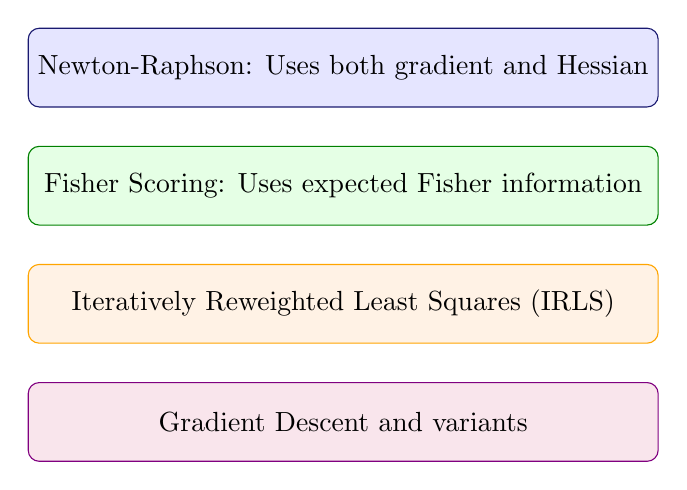
\begin{tikzpicture}[node distance=1.5cm]
\tikzstyle{method} = [rectangle, rounded corners, minimum width=8cm, minimum height=1cm, text centered]

\node (M1) [method, draw=MidnightBlue, fill=blue!10] {Newton-Raphson: Uses both gradient and Hessian};
\node (M2) [method, below of=M1, draw=Green, fill=green!10] {Fisher Scoring: Uses expected Fisher information};
\node (M3) [method, below of=M2, draw=Orange, fill=orange!10] {Iteratively Reweighted Least Squares (IRLS)};
\node (M4) [method, below of=M3, draw=Purple, fill=purple!10] {Gradient Descent and variants};
\end{tikzpicture}
\end{center}
\end{frame}

\begin{frame}{Newton-Raphson Algorithm}
The Newton-Raphson method uses a quadratic approximation:

\begin{block}{Update Formula}
$$\beta^{(t+1)} = \beta^{(t)} - \mathbf{H}^{-1}(\beta^{(t)}) U(\beta^{(t)})$$
\end{block}

\begin{block}{Logistic Regression Update}
Substituting $U$ and $\mathbf{H}$:
$$\beta^{(t+1)} = \beta^{(t)} + (\mathbf{X}^T \mathbf{W}^{(t)} \mathbf{X})^{-1} \mathbf{X}^T (\mathbf{y} - \boldsymbol{\pi}^{(t)})$$
where $\mathbf{W}^{(t)} = \text{diag}\{\pi_1^{(t)}(1-\pi_1^{(t)}), \ldots\}$ and $\pi_i^{(t)}$ is the predicted probability at iteration $t$.
\end{block}

\begin{block}{Algorithm Steps}
\begin{enumerate}
\item Initialize $\beta^{(0)}$ (often with $\beta = 0$)
\item Compute $\pi_i^{(t)}$ and $\mathbf{W}^{(t)}$
\item Compute the update $\Delta\beta = (\mathbf{X}^T \mathbf{W}^{(t)} \mathbf{X})^{-1} \mathbf{X}^T (\mathbf{y} - \boldsymbol{\pi}^{(t)})$
\item Update $\beta^{(t+1)} = \beta^{(t)} + \Delta\beta$
\item Repeat until convergence (when $\|\Delta\beta\| < \epsilon$)
\end{enumerate}
\end{block}
\end{frame}

\begin{frame}{Fisher Scoring (IRLS) Method}
Fisher Scoring uses the expected Fisher information (expected Hessian):

\begin{block}{Fisher Information Matrix}
The observed Fisher information is $-\mathbf{H} = \mathbf{X}^T \mathbf{W} \mathbf{X}$. The expected Fisher information is the same for logistic regression.
\end{block}

\begin{block}{IRLS Interpretation}
The update equation resembles weighted least squares:
$$\beta^{(t+1)} = (\mathbf{X}^T \mathbf{W}^{(t)} \mathbf{X})^{-1} \mathbf{X}^T \mathbf{W}^{(t)} \mathbf{z}^{(t)}$$
where the working response $\mathbf{z}^{(t)}$ is:
$$z_i^{(t)} = X_i^T\beta^{(t)} + \frac{y_i - \pi_i^{(t)}}{\pi_i^{(t)}(1-\pi_i^{(t)})}$$
\end{block}

\begin{block}{Convergence}
Typically converges in 5-10 iterations. The IRLS method is computationally efficient and forms the basis for many software implementations.
\end{block}
\end{frame}

\begin{frame}{Interpreting Newton-Raphson: A Simple Example}
Consider a single predictor $X$ with true $\beta = (0.5, 1.0)^T$:

\begin{center}
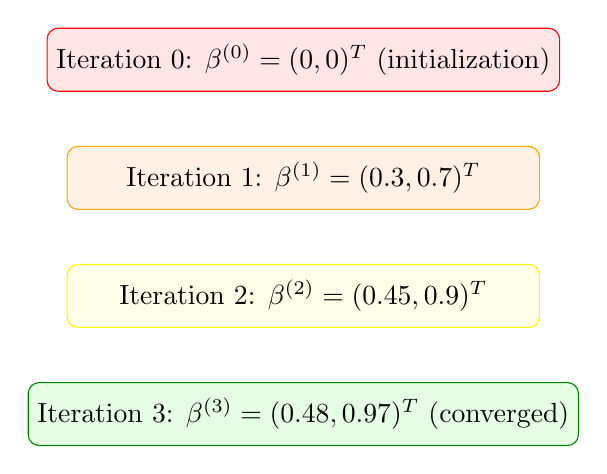
\begin{tikzpicture}[node distance=1.5cm]
\tikzstyle{iter} = [rectangle, rounded corners, minimum width=6cm, minimum height=0.8cm, text centered]

\node (I0) [iter, draw=Red, fill=red!10] {Iteration 0: $\beta^{(0)} = (0, 0)^T$ (initialization)};
\node (I1) [iter, below of=I0, draw=Orange, fill=orange!10] {Iteration 1: $\beta^{(1)} = (0.3, 0.7)^T$};
\node (I2) [iter, below of=I1, draw=Yellow, fill=yellow!10] {Iteration 2: $\beta^{(2)} = (0.45, 0.9)^T$};
\node (I3) [iter, below of=I2, draw=Green, fill=green!10] {Iteration 3: $\beta^{(3)} = (0.48, 0.97)^T$ (converged)};
\end{tikzpicture}
\end{center}

\begin{block}{Visualization of Convergence}
The algorithm "climbs" the log-likelihood surface, with step sizes determined by the curvature (Hessian). Near the maximum, steps become smaller.
\end{block}
\end{frame}

\begin{frame}{Assessing Convergence}
Proper convergence assessment is crucial:

\begin{block}{Convergence Criteria}
\begin{itemize}
\item \textbf{Parameter change:} $\|\beta^{(t+1)} - \beta^{(t)}\| < 10^{-5}$
\item \textbf{Score change:} $\|U(\beta^{(t)})\| < 10^{-5}$
\item \textbf{Log-likelihood change:} $|\ell(\beta^{(t+1)}) - \ell(\beta^{(t)})| < 10^{-5}$
\end{itemize}
\end{block}

\begin{block}{Potential Issues}
\begin{itemize}
\item \textbf{Separation:} When a predictor perfectly predicts the outcome, coefficients diverge to $\pm\infty$
\item \textbf{Quasi-separation:} Near-perfect prediction causes numerical instability
\item \textbf{Sparse data:} With few events per predictor, estimates may be unstable
\end{itemize}
\end{block}

\begin{block}{Remedies}
\begin{itemize}
\item Firth's penalized likelihood (bias reduction)
\item Regularization (ridge, LASSO)
\end{itemize}
\end{block}
\end{frame}

\begin{frame}{Variance Estimation}
After convergence, the variance-covariance matrix is estimated:

\begin{block}{Observed Fisher Information}
$$\widehat{\text{Cov}}(\hat{\beta}) = (-\mathbf{H}(\hat{\beta}))^{-1} = (\mathbf{X}^T \hat{\mathbf{W}} \mathbf{X})^{-1}$$
where $\hat{\mathbf{W}} = \text{diag}\{\hat{\pi}_1(1-\hat{\pi}_1), \ldots, \hat{\pi}_n(1-\hat{\pi}_n)\}$.
\end{block}

\begin{block}{Standard Errors}
The standard error of $\hat{\beta}_j$ is:
$$\text{SE}(\hat{\beta}_j) = \sqrt{\widehat{\text{Cov}}(\hat{\beta})_{jj}}$$
\end{block}

\begin{block}{Wald Tests}
For testing $H_0: \beta_j = 0$:
$$z = \frac{\hat{\beta}_j}{\text{SE}(\hat{\beta}_j)} \sim \mathcal{N}(0,1) \quad \text{(asymptotically)}$$
or equivalently, $\chi^2 = z^2$ with 1 degree of freedom.
\end{block}
\end{frame}

% ============================================================================
% SECTION 5: INTERPRETING LOGISTIC REGRESSION COEFFICIENTS
% ============================================================================

\section{Interpreting Estimated Coefficients}

\subsection{Odds Ratios}

\begin{frame}{The Odds Ratio as a Measure of Association}
The coefficient $\beta_j$ represents the change in log-odds per unit change in $X_j$:

\begin{block}{Interpretation of $\beta_j$}
For a one-unit increase in predictor $X_j$ (holding other predictors constant):
$$\log\left(\frac{\text{odds}(Y=1|X_j+1)}{\text{odds}(Y=1|X_j)}\right) = \beta_j$$
Thus, $\beta_j$ is the log-odds ratio comparing the odds when $X_j$ increases by 1.
\end{block}

\begin{block}{Odds Ratio Interpretation}
The odds ratio (OR) is the exponential transformation:
$$\text{OR} = e^{\beta_j} = \frac{\text{odds}(Y=1|X_j+1)}{\text{odds}(Y=1|X_j)}$$
\end{block}

\begin{center}
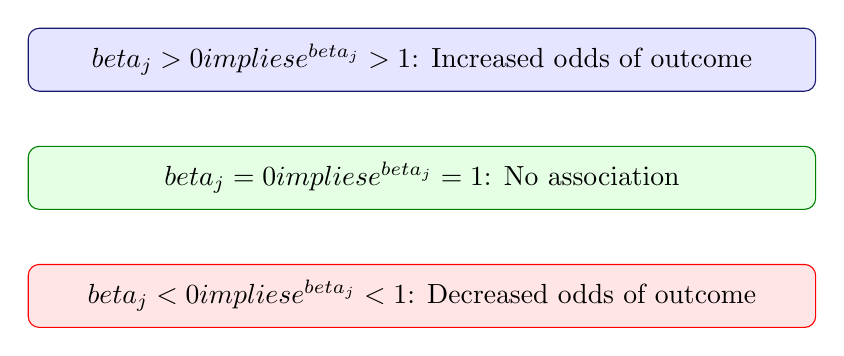
\begin{tikzpicture}[node distance=1.5cm]
\tikzstyle{interpret} = [rectangle, rounded corners, minimum width=10cm, minimum height=0.8cm, text centered]

\node (I1) [interpret, draw=MidnightBlue, fill=blue!10] {$\\beta_j > 0 \\implies e^{\\beta_j} > 1$: Increased odds of outcome};
\node (I2) [interpret, below of=I1, draw=Green, fill=green!10] {$\\beta_j = 0 \\implies e^{\\beta_j} = 1$: No association};
\node (I3) [interpret, below of=I2, draw=Red, fill=red!10] {$\\beta_j < 0 \\implies e^{\\beta_j} < 1$: Decreased odds of outcome};
\end{tikzpicture}
\end{center}
\end{frame}

\begin{frame}{Example: Odds Ratio Calculation}
Consider a model predicting diabetes status from age:

\begin{block}{Model}
$$\log\left(\frac{P(\text{Diabetes}=1)}{1-P(\text{Diabetes}=1)}\right) = \beta_0 + \beta_1 \cdot \text{Age}$$
\end{block}

\begin{block}{Estimated Coefficients}
Suppose $\hat{\beta}_0 = -5.0$ and $\hat{\beta}_1 = 0.08$.
\end{block}

\begin{block}{Interpretation}
\begin{itemize}
\item For a 1-year increase in age: $\text{OR} = e^{0.08} = 1.083$
\item Interpretation: Each additional year of age is associated with an 8.3\% increase in the odds of diabetes.
\item For a 10-year increase: $\text{OR} = e^{0.08 \times 10} = e^{0.8} = 2.23$
\end{itemize}
\end{block}

\begin{block}{Confidence Interval}
If $\text{SE}(\hat{\beta}_1) = 0.02$, then a 95\% CI for $\beta_1$ is:
$$0.08 \pm 1.96 \times 0.02 = (0.039, 0.121)$$
Exponentiating gives a 95\% CI for the OR: $(1.04, 1.13)$.
\end{block}
\end{frame}

\begin{frame}{Continuous Predictors: Unit Changes}
The interpretation depends on the chosen unit of measurement:

\begin{block}{Standardized Coefficients}
Standardizing $X_j$ to have unit variance allows comparison of relative importance:
$$\hat{\beta}_j^{\text{std}} = \hat{\beta}_j \times \text{SD}(X_j)$$
Then $e^{\hat{\beta}_j^{\text{std}}}$ represents the OR per one SD change in $X_j$.
\end{block}

\begin{block}{Interpretation Guidelines}
\begin{itemize}
\item Report ORs for meaningful unit changes (not just per 1 unit)
\item Consider whether the unit change is substantively meaningful
\end{itemize}
\end{block}

\begin{block}{Example}
If blood pressure is measured in mmHg, report the OR per 10 mmHg or 20 mmHg change rather than per 1 mmHg.
\end{block}
\end{frame}

\begin{frame}{Categorical Predictors: Reference Categories}
For categorical predictors, one coefficient per category compares to a reference:

\begin{block}{Example: Smoking Status and Lung Cancer}
\begin{center}
\begin{tabular}{lcc}
\toprule
Smoking Status & $\hat{\beta}$ & OR ($e^{\hat{\beta}}$) \\
\midrule
Never (Reference) & 0 & 1.0 \\
Former & 0.85 & 2.34 \\
Current & 2.10 & 8.17 \\
\bottomrule
\end{tabular}
\end{center}
\end{block}

\begin{block}{Interpretation}
Current smokers have 8.17 times higher odds of lung cancer compared to never smokers (95\% CI: 5.12-13.0), adjusting for other factors.
\end{block}
\end{frame}

\begin{frame}{Interaction Terms}
When predictors interact, the effect of one depends on the level of the other:

\begin{block}{Model with Interaction}
$$\log\left(\frac{P(Y=1)}{1-P(Y=1)}\right) = \beta_0 + \beta_1 X_1 + \beta_2 X_2 + \beta_3 X_1 X_2$$
\end{block}

\begin{block}{Interpretation of $\beta_3$}
$\beta_3$ represents the additional change in log-odds for a unit increase in $X_1$ when $X_2$ increases by 1. The OR for the interaction is $e^{\beta_3}$.
\end{block}

\begin{block}{Caveat}
Never interpret main effects ($\beta_1, \beta_2$) in isolation when an interaction is present. They represent effects when the other predictor is at its reference level (for categorical) or zero (for continuous).
\end{block}
\end{frame}

% ============================================================================
% SECTION 6: APPLICATIONS IN PUBLIC HEALTH
% ============================================================================

\section{Applications in Public Health and Disease Risk Modeling}

\begin{frame}{Logistic Regression in Epidemiology}
Logistic regression is widely used for studying disease risk factors:

\begin{center}
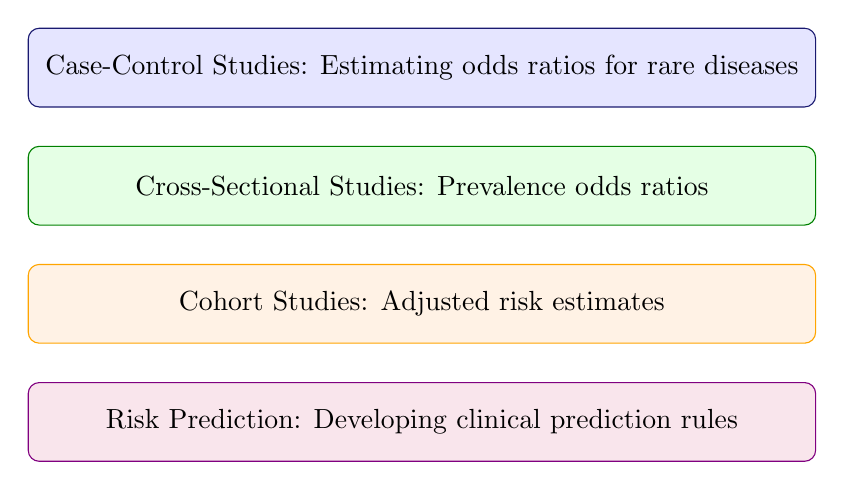
\begin{tikzpicture}[node distance=1.5cm]
\tikzstyle{application} = [rectangle, rounded corners, minimum width=10cm, minimum height=1cm, text centered]

\node (A1) [application, draw=MidnightBlue, fill=blue!10] {Case-Control Studies: Estimating odds ratios for rare diseases};
\node (A2) [application, below of=A1, draw=Green, fill=green!10] {Cross-Sectional Studies: Prevalence odds ratios};
\node (A3) [application, below of=A2, draw=Orange, fill=orange!10] {Cohort Studies: Adjusted risk estimates};
\node (A4) [application, below of=A3, draw=Purple, fill=purple!10] {Risk Prediction: Developing clinical prediction rules};
\end{tikzpicture}
\end{center}
\end{frame}

\begin{frame}{Example: Risk Factors for Cardiovascular Disease}
A prospective cohort study examines multiple risk factors:

\begin{block}{Model}
\begin{align*}
\log\left(\frac{P(\text{CVD}=1)}{1-P(\text{CVD}=1)}\right) &= \beta_0 + \beta_1 \cdot \text{Age} + \beta_2 \cdot \text{Male} + \beta_3 \cdot \text{SBP} \\
                                                          &\quad + \beta_4 \cdot \text{Smoker} + \beta_5 \cdot \text{Diabetes}
\end{align*}
\end{block}

\begin{block}{Sample Results}
\begin{center}
\begin{tabular}{lccc}
\toprule
Predictor & $\hat{\beta}$ & OR & 95\% CI \\
\midrule
Age (per 10 years) & 0.72 & 2.05 & (1.85, 2.28) \\
Male (vs. Female) & 0.45 & 1.57 & (1.32, 1.86) \\
SBP (per 20 mmHg) & 0.38 & 1.46 & (1.31, 1.63) \\
Current Smoker & 0.89 & 2.44 & (2.05, 2.90) \\
Diabetes & 1.12 & 3.06 & (2.51, 3.73) \\
\bottomrule
\end{tabular}
\end{center}
\end{block}
\end{frame}

\begin{frame}{Clinical Risk Prediction Models}
Logistic regression forms the basis for many clinical prediction tools:

\begin{block}{Framingham Risk Score}
Estimates 10-year cardiovascular disease risk using logistic regression coefficients.
\end{block}

\begin{block}{Components of Risk Prediction Models}
\begin{itemize}
\item \textbf{Development:} Fit logistic regression on derivation cohort
\item \textbf{Validation:} Assess performance in independent samples
\item \textbf{Calibration:} Do predicted probabilities match observed frequencies?
\item \textbf{Discrimination:} Can the model distinguish high vs. low risk? (C-statistic)
\end{itemize}
\end{block}

\begin{block}{Performance Metrics}
\begin{center}
\begin{tabular}{ll}
\toprule
Metric & Interpretation \\
\midrule
C-statistic (AUC) & 0.5 = random, 1.0 = perfect \\
Calibration slope & 1 = well-calibrated, <1 = overfitting \\
Brier score & Lower = better \\
\bottomrule
\end{tabular}
\end{center}
\end{block}
\end{frame}

\begin{frame}{Advantages of MLE-Based Logistic Regression}
\begin{columns}
\begin{column}{0.5\textwidth}
\begin{block}{Statistical Properties}
\begin{itemize}
\item Consistent and asymptotically efficient
\item Well-underposed theoretical properties
\item Confidence intervals readily available
\end{itemize}
\end{block}
\end{column}
\begin{column}{0.5\textwidth}
\begin{block}{Practical Advantages}
\begin{itemize}
\item Handles multiple predictors naturally
\item Can model continuous and categorical predictors
\end{itemize}
\end{block}
\end{column}
\end{columns}

\begin{block}{Extensions}
\begin{center}
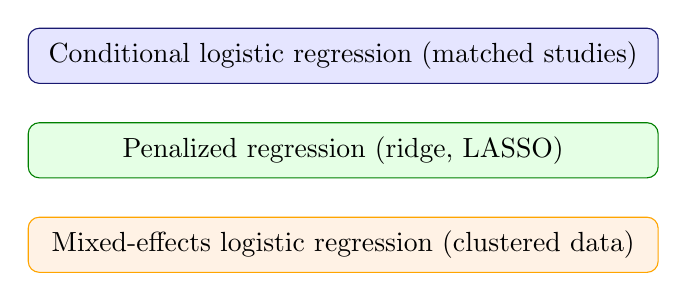
\begin{tikzpicture}[node distance=1.2cm]
\tikzstyle{extend} = [rectangle, rounded corners, minimum width=8cm, minimum height=0.7cm, text centered]

\node (E1) [extend, draw=MidnightBlue, fill=blue!10] {Conditional logistic regression (matched studies)};
\node (E2) [extend, below of=E1, draw=Green, fill=green!10] {Penalized regression (ridge, LASSO)};
\node (E3) [extend, below of=E2, draw=Orange, fill=orange!10] {Mixed-effects logistic regression (clustered data)};
\end{tikzpicture}
\end{center}
\end{block}
\end{frame}

\begin{frame}{Limitations and Considerations}
\begin{columns}
\begin{column}{0.5\textwidth}
\begin{block}{Model Assumptions}
\begin{itemize}
\item Linearity in the log-odds
\item Independence of observations
\end{itemize}
\end{block}
\begin{block}{Sample Size Requirements}
\begin{itemize}
\item Rule of thumb: 10-20 events per predictor
\end{itemize}
\end{block}
\end{column}
\begin{column}{0.5\textwidth}
\begin{block}{Limitations}
\begin{itemize}
\item Odds ratios can be misinterpreted as risk ratios
\end{itemize}
\end{block}
\begin{block}{Alternatives When OR $\neq$ RR}
\begin{center}

\begin{tikzpicture}[node distance=1cm]
\tikzstyle{alt} = [rectangle, rounded corners, minimum width=7cm, minimum height=0.6cm, text centered]

\node (A1) [alt, draw=Red, fill=red!10] {When outcome is common (>10\%): Use log-binomial or Poisson regression};
\end{tikzpicture}
\end{center}
\end{block}
\end{column}
\end{columns}
\end{frame}

% ============================================================================
% SECTION 7: CONCLUSION
% ============================================================================

\section{Conclusion and Key Takeaways}

\begin{frame}{Summary: MLE and Logistic Regression}
\begin{center}
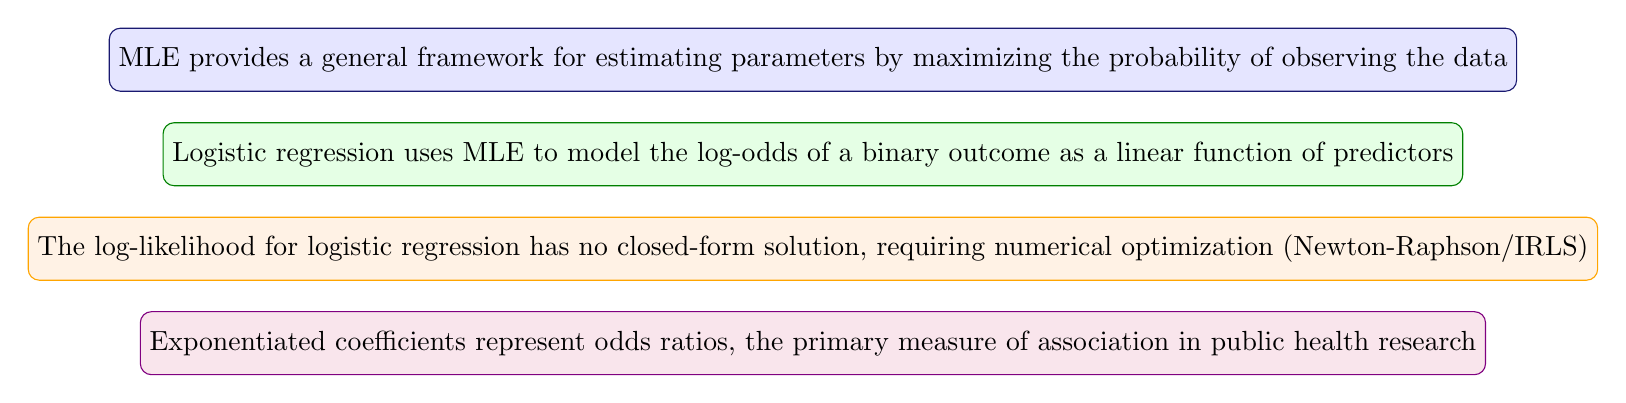
\begin{tikzpicture}[node distance=1.2cm]
\tikzstyle{summary} = [rectangle, rounded corners, minimum width=10cm, minimum height=0.8cm, text centered]

\node (S1) [summary, draw=MidnightBlue, fill=blue!10] {MLE provides a general framework for estimating parameters by maximizing the probability of observing the data};
\node (S2) [summary, below of=S1, draw=Green, fill=green!10] {Logistic regression uses MLE to model the log-odds of a binary outcome as a linear function of predictors};
\node (S3) [summary, below of=S2, draw=Orange, fill=orange!10] {The log-likelihood for logistic regression has no closed-form solution, requiring numerical optimization (Newton-Raphson/IRLS)};
\node (S4) [summary, below of=S3, draw=Purple, fill=purple!10] {Exponentiated coefficients represent odds ratios, the primary measure of association in public health research};
\end{tikzpicture}
\end{center}
\end{frame}

\begin{frame}{Key Equations Summary}
\begin{center}
\begin{small}
\begin{align*}
\textbf{Logistic Model:} \quad & P(Y=1|X) = \frac{1}{1 + e^{-(\beta_0 + \beta_1 X_1 + \cdots + \beta_k X_k)}} \\
\textbf{Log-Odds:} \quad & \log\left(\frac{P(Y=1|X)}{1-P(Y=1|X)}\right) = \beta_0 + \beta_1 X_1 + \cdots + \beta_k X_k \\
\textbf{Log-Likelihood:} \quad & \ell(\beta) = \sum_{i=1}^{n} \left[y_i X_i^T\beta - \log(1 + e^{X_i^T\beta})\right] \\
\textbf{Score Function:} \quad & U_j(\beta) = \sum_{i=1}^{n} X_{ij}(y_i - \pi_i) \\
\textbf{Odds Ratio:} \quad & \text{OR} = e^{\beta_j} \quad \text{(for 1-unit change in } X_j\text{)}
\end{align*}
\end{small}
\end{center}
\end{frame}

\begin{frame}{Final Takeaways for Public Health Practice}
\begin{columns}
\begin{column}{0.5\textwidth}
\begin{block}{Strengths of MLE Logistic Regression}
\begin{itemize}
\item Interpretable odds ratios
\item Well-established statistical properties
\item Widely implemented in statistical software
\end{itemize}
\end{block}
\end{column}
\begin{column}{0.5\textwidth}
\begin{block}{Best Practices}
\begin{itemize}
\item Check model assumptions
\item Assess model fit and discrimination
\end{itemize}
\end{block}
\end{column}
\end{columns}

\begin{center}
\textbf{"Logistic regression remains a cornerstone of epidemiologic analysis for binary outcomes, providing both etiologic insight through odds ratios and clinical utility through risk prediction."}
\end{center}
\end{frame}

\begin{frame}{References}
\begin{small}
\begin{itemize}
\item Hosmer, D.W., Lemeshow, S., \& Sturdivant, R.X. (2013). Applied Logistic Regression (3rd ed.). Wiley.
\item Agresti, A. (2018). An Introduction to Categorical Data Analysis (3rd ed.). Wiley.
\item McCullagh, P. \& Nelder, J.A. (1989). Generalized Linear Models (2nd ed.). Chapman \& Hall.
\item Rothman, K.J., Greenland, S., \& Lash, T.L. (2008). Modern Epidemiology (3rd ed.). Lippincott Williams \& Wilkins.
\end{itemize}
\end{small}
\end{frame}

\end{document}
